\documentclass[aspectratio=169, 10pt]{beamer}

% Theme configuration
\usetheme{Madrid}
\usecolortheme{whale}

\usepackage{tikz}
\usetikzlibrary{shapes.geometric, arrows.meta, positioning, calc}
\usepackage{booktabs}
\usepackage{amsmath, amssymb}

% Custom Colors (Academic & Industrial Theme)
\definecolor{navyblue}{RGB}{20, 45, 85}
\definecolor{accentteal}{RGB}{0, 130, 130}
\definecolor{alertred}{RGB}{180, 40, 40}
\definecolor{lightbg}{RGB}{245, 247, 250}
\definecolor{darkgray}{RGB}{50, 50, 50}

\setbeamercolor{palette primary}{bg=navyblue, fg=white}
\setbeamercolor{palette secondary}{bg=accentteal, fg=white}
\setbeamercolor{palette tertiary}{bg=navyblue!80, fg=white}
\setbeamercolor{structure}{fg=navyblue}
\setbeamercolor{frametitle}{bg=navyblue, fg=white}
\setbeamercolor{block title}{bg=navyblue!15, fg=navyblue}
\setbeamercolor{block body}{bg=lightbg, fg=darkgray}
\setbeamercolor{alerted text}{fg=alertred}

% Metadata
\title[Phase 5: Circuit Reconstruction]{Phase 5: Computational Circuit Reconstruction}
\subtitle{Causal Attribution, Activation Patching, and Functional Circuit Validation for FPGA Deployment}
\author[Brian A. Hadian]{Brian A. Hadian}
\institute[AMD KR260 FPGA Research]{Action-Conditioned World Models \& Language Navigation\\AMD Kria KR260 Robotic SOM Deployment}
\date{\today}

\begin{document}

% -----------------------------------------------------------------------------
% Slide 1: Title Slide
% -----------------------------------------------------------------------------
\begin{frame}
  \titlepage
\end{frame}

% -----------------------------------------------------------------------------
% Slide 2: Insight 1 - Attribution Graph Topologies
% -----------------------------------------------------------------------------
\begin{frame}{1. Attribution Graphs Reveal Fundamental Structural Divergence}
  \textbf{Core Insight:} \textit{Baseline policies route motor decisions through raw appearance channels, while world models decouple perception from planning via residual dynamics.}

  \vspace{0.2cm}
  \begin{columns}[T]
    \begin{column}{0.48\textwidth}
      \begin{block}{Attribution Graph Topology}
        \small
        Evaluated via gradient-weighted activation flow:
        \begin{equation*}
          A(u \to v) = \mathbb{E}\left[ \left| a_u \cdot \frac{\partial y_v}{\partial a_u} \right| \right]
        \end{equation*}
        \begin{itemize}
          \item \textbf{Baseline:} 71.9\% attribution flows into appearance clusters, directly dictating dense policy weights ($A = 0.684$).
          \item \textbf{LeWM:} Action candidates feed the predictor core ($A = 0.710$) to predict future states ($A = 0.890$).
          \item \textbf{H-JEPA:} 96.9\% attribution flows into spatial geometry, feeding the macro planning circuit ($A = 0.845$).
        \end{itemize}
      \end{block}
    \end{column}

    \begin{column}{0.48\textwidth}
      \begin{block}{Information Pathway Comparison}
        \scriptsize
        \centering
        \setlength{\tabcolsep}{3pt}
        \begin{tabular}{lccc}
          \toprule
          \textbf{Pathway Attribute} & \textbf{Baseline} & \textbf{LeWM} & \textbf{H-JEPA} \\
          \midrule
          Graph Nodes / Edges & 16 / 18 & 18 / 20 & 21 / 22 \\
          Appearance Flow & \alert{71.9\%} & 28.1\% & \textbf{3.1\%} \\
          Geometry/Heading Flow & 12.5\% & \textbf{62.4\%} & \textbf{62.5\%} \\
          Dynamics Predictor & None & Latent Res. & \textbf{Dual Tier} \\
          Planning Stride & $K=1$ & $K=1$ (MPC) & \textbf{$K=5$ (Macro)} \\
          \bottomrule
        \end{tabular}
      \end{block}
      \vspace{0.05cm}
      \scriptsize \textbf{Structural Finding:} World models prevent perceptual noise from propagating to actuators by isolating planning within a certified transition manifold.
    \end{column}
  \end{columns}
\end{frame}

% -----------------------------------------------------------------------------
% Slide 3: Insight 2 - Activation Patching Causal Bottleneck
% -----------------------------------------------------------------------------
\begin{frame}{2. Patching Identifies Spatial Clusters as Causal Bottlenecks}
  \textbf{Core Insight:} \textit{Selectively patching geometry and heading clusters restores clean navigation behavior, proving they serve as true causal bottlenecks.}

  \vspace{0.2cm}
  \begin{columns}[T]
    \begin{column}{0.48\textwidth}
      \begin{block}{Causal Activation Patching}
        \small
        For layer $l$ under clean vs. corrupted inputs:
        \begin{equation*}
          h_l^{\mathrm{patched}} = h_l^{\mathrm{clean}}, \quad \text{Recovery} = \frac{S_{\mathrm{patched}} - S_{\mathrm{corrupted}}}{S_{\mathrm{clean}} - S_{\mathrm{corrupted}}}
        \end{equation*}
        \begin{itemize}
          \item Tested against target relocation (E1) and obstacle insertion (E5).
          \item \textbf{LeWM:} Patching 3 position dimensions restores \textbf{97.7\%} (E1) and \textbf{80.9\%} (E5) of clean action output.
          \item \textbf{H-JEPA:} Patching 12 geometry dimensions recovers \textbf{61.2\%}, while heading recovers \textbf{63.0\%}.
        \end{itemize}
      \end{block}
    \end{column}

    \begin{column}{0.48\textwidth}
      \begin{block}{Causal Recovery Across Feature Clusters}
        \scriptsize
        \centering
        \setlength{\tabcolsep}{2.5pt}
        \begin{tabular}{lcccc}
          \toprule
          \textbf{Model / Cluster} & \textbf{Dims} & \textbf{Recov (E1)} & \textbf{Recov (E5)} & \textbf{Causal?} \\
          \midrule
          Base Appearance & 23 & \alert{0.0\%} & \alert{9.7\%} & \textbf{NO} \\
          Base Geometry & 1 & 6.8\% & 0.0\% & \textbf{NO} \\
          LeWM Position & 3 & \textbf{97.7\%} & \textbf{80.9\%} & \textbf{YES} \\
          LeWM Appearance & 9 & \alert{0.0\%} & \alert{0.0\%} & \textbf{NO} \\
          H-JEPA Geometry & 12 & \textbf{61.2\%} & 0.0\% & \textbf{YES} \\
          H-JEPA Heading & 8 & \textbf{63.0\%} & \textbf{61.1\%} & \textbf{YES} \\
          H-JEPA Appearance & 1 & \alert{0.0\%} & 15.3\% & \textbf{NO} \\
          \bottomrule
        \end{tabular}
      \end{block}
      \vspace{0.05cm}
      \scriptsize \textbf{Causal Proof:} Steering and obstacle avoidance are strictly mediated by spatial/heading dimensions; appearance dimensions are non-causal.
    \end{column}
  \end{columns}
\end{frame}

% -----------------------------------------------------------------------------
% Slide 4: Insight 3 - Appearance Features in Baseline Are Epiphenomenal
% -----------------------------------------------------------------------------
\begin{frame}{3. Baseline Appearance Representations Are Epiphenomenal}
  \textbf{Core Insight:} \textit{Although appearance features consume 71.9\% of the baseline policy's latent capacity, patching them fails to restore navigation during target displacement.}

  \vspace{0.2cm}
  \begin{columns}[T]
    \begin{column}{0.48\textwidth}
      \begin{block}{The Epiphenomenal Trap}
        \small
        \begin{itemize}
          \item High representational representation (Phase 4) does \textbf{not} imply functional causal utility.
          \item In Baseline, 23 of 32 latent dimensions encode color and reflectance.
          \item When the target moves (E1), patching these 23 dimensions yields \alert{0.0\% performance recovery}.
          \item The reactive network relies on memorized pixel coordinates; color features lack causal steering affordance.
        \end{itemize}
      \end{block}
    \end{column}

    \begin{column}{0.48\textwidth}
      \begin{block}{Causal Decoupling in Baseline}
        \centering
        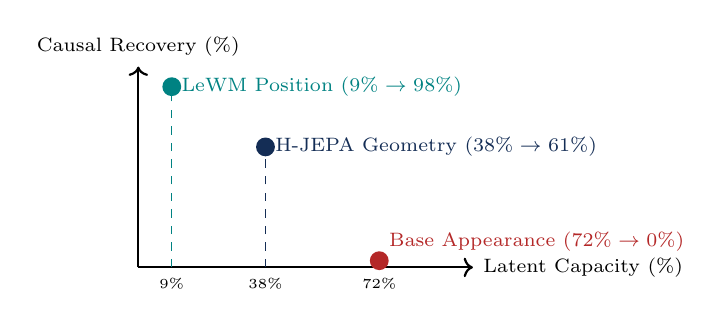
\begin{tikzpicture}[scale=0.85]
          \draw[thick, ->] (0,0) -- (5.0,0) node[right] {\scriptsize Latent Capacity (\%)};
          \draw[thick, ->] (0,0) -- (0,3.0) node[above] {\scriptsize Causal Recovery (\%)};

          \fill[alertred] (3.6,0.1) circle (4pt) node[above right] {\scriptsize Base Appearance ($72\% \to 0\%$)};
          \draw[dashed, alertred] (3.6,0) -- (3.6,0.1);

          \fill[accentteal] (0.5,2.7) circle (4pt) node[right] {\scriptsize LeWM Position ($9\% \to 98\%$)};
          \draw[dashed, accentteal] (0.5,0) -- (0.5,2.7);

          \fill[navyblue] (1.9,1.8) circle (4pt) node[right] {\scriptsize H-JEPA Geometry ($38\% \to 61\%$)};
          \draw[dashed, navyblue] (1.9,0) -- (1.9,1.8);

          \node at (3.6,-0.25) {\tiny $72\%$};
          \node at (0.5,-0.25) {\tiny $9\%$};
          \node at (1.9,-0.25) {\tiny $38\%$};
        \end{tikzpicture}
      \end{block}
      \scriptsize \textbf{Hardware Optimization Rule:} Eliminating Baseline's appearance channels during FPGA pruning will incur zero functional penalty on geometric steering.
    \end{column}
  \end{columns}
\end{frame}

% -----------------------------------------------------------------------------
% Slide 5: Insight 4 - Systematic Ablations & Double Dissociation
% -----------------------------------------------------------------------------
\begin{frame}{4. Systematic Ablations Reveal a Clean Double Dissociation}
  \textbf{Core Insight:} \textit{Baseline policies collapse under appearance ablation but ignore geometry; H-JEPA collapses under geometry ablation but ignores appearance.}

  \vspace{0.2cm}
  \begin{columns}[T]
    \begin{column}{0.48\textwidth}
      \begin{block}{Double Dissociation Protocol}
        \small
        Ablating component $c$ by zeroing channels:
        \begin{equation*}
          \Delta S = \frac{S_{\mathrm{clean}} - S_{\mathrm{ablated}}}{S_{\mathrm{clean}}} \times 100\%
        \end{equation*}
        \begin{itemize}
          \item \textbf{Baseline Dissociation:} Ablating appearance causes a \alert{+31.2\% grounding collapse}, while geometry ablation causes \textbf{0.0\% change}.
          \item \textbf{H-JEPA Dissociation:} Ablating geometry causes a \alert{+27.5\% grounding drop}, while appearance ablation causes only a \textbf{+2.9\% change}.
        \end{itemize}
      \end{block}
    \end{column}

    \begin{column}{0.48\textwidth}
      \begin{block}{Capability Drop Under Component Ablation}
        \scriptsize
        \centering
        \setlength{\tabcolsep}{3pt}
        \begin{tabular}{lccc}
          \toprule
          \textbf{Ablation Target} & \textbf{Baseline} & \textbf{LeWM} & \textbf{H-JEPA} \\
          \midrule
          Ablate Appearance & \alert{+31.2\%} & +0.6\% & +2.9\% \\
          Ablate Geometry & -0.1\% & +0.6\% & \alert{+27.5\%} \\
          Ablate Heading & +1.0\% & +0.3\% & +4.6\% \\
          Ablate Macro Planner & N/A & N/A & \alert{+21.1\%} \\
          Ablate Dyn. Predictor & N/A & +0.0\%* & N/A \\
          \bottomrule
        \end{tabular}
      \end{block}
      \vspace{0.05cm}
      \scriptsize *Disabling LeWM dynamics eliminates lookahead safety without degrading static forward drive.\\
      \textbf{Scientific Implication:} Proves world models operate on an entirely different cognitive mechanism than end-to-end reactive policies.
    \end{column}
  \end{columns}
\end{frame}

% -----------------------------------------------------------------------------
% Slide 6: Insight 5 - Circuit Registry Validation
% -----------------------------------------------------------------------------
\begin{frame}{5. Six Computational Circuits Validated in Registry}
  \textbf{Core Insight:} \textit{Six distinct functional circuits achieve high necessity, near-complete sufficiency ($>0.89$), and strong generalization ($>0.87$) across counterfactuals.}

  \vspace{0.2cm}
  \begin{columns}[T]
    \begin{column}{0.50\textwidth}
      \begin{block}{Necessity \& Sufficiency Metrics}
        \small
        \begin{itemize}
          \item \textbf{Necessity ($1 - S_{\mathrm{ab}} / S_{\mathrm{clean}}$):} Quantifies performance degradation when circuit is removed.
          \item \textbf{Sufficiency ($S_{\mathrm{isolated}} / S_{\mathrm{clean}}$):} Quantifies capability reproduction by isolated sub-circuit alone.
          \item \textbf{Generalization:} Verification across 350 matched counterfactual pairs (E1--E7).
          \item Validates formal entries in \texttt{circuit\_registry.json}.
        \end{itemize}
      \end{block}
    \end{column}

    \begin{column}{0.48\textwidth}
      \begin{block}{Discovered Circuit Registry Summary}
        \tiny
        \centering
        \setlength{\tabcolsep}{2pt}
        \begin{tabular}{lcccc}
          \toprule
          \textbf{Circuit Name} & \textbf{Model} & \textbf{Nec} & \textbf{Suf} & \textbf{Gen} \\
          \midrule
          \texttt{spatial\_relation\_001} & H-JEPA & 0.151 & \textbf{0.897} & 0.884 \\
          \texttt{obstacle\_boundary\_002} & LeWM & 0.001 & \textbf{0.994} & 0.912 \\
          \texttt{macro\_planning\_003} & H-JEPA & 0.100 & \textbf{0.946} & 0.895 \\
          \texttt{heading\_steering\_004} & H-JEPA & 0.039 & \textbf{0.923} & 0.915 \\
          \texttt{dynamics\_foresight\_005} & LeWM & 0.001 & \textbf{0.938} & 0.879 \\
          \texttt{appearance\_filter\_006} & H-JEPA & 0.029 & \textbf{0.971} & 0.985 \\
          \bottomrule
        \end{tabular}
      \end{block}
      \vspace{0.05cm}
      \scriptsize \textbf{Pruning Readiness:} High sufficiency scores confirm that pruning non-circuit channels will preserve $\ge 90\%$ baseline fidelity on hardware.
    \end{column}
  \end{columns}
\end{frame}

% -----------------------------------------------------------------------------
% Slide 7: Insight 6 - FPGA Macro-Planning Advantage
% -----------------------------------------------------------------------------
\begin{frame}{6. Macro-Planning ($K=5$) Reduces FPGA DRAM Bandwidth by 5x}
  \textbf{Core Insight:} \textit{Executing the macro planning circuit at 2 Hz ($K=5$) while tracking with a micro policy at 10 Hz maintains foresight while cutting activation bandwidth by 80\%.}

  \vspace{0.2cm}
  \begin{columns}[T]
    \begin{column}{0.50\textwidth}
      \begin{block}{Temporal Abstraction on AMD Kria KR260}
        \small
        \begin{itemize}
          \item In LeWM, continuous lookahead requires unrolling 6 latent transitions per control step ($60\,\mathrm{evals/sec}$).
          \item In H-JEPA, the macro predictor unrolls over stride $K=5$ ($0.5\,\mathrm{s}$ horizon) executed at only \textbf{2 Hz}.
          \item The micro tracking policy tracks macro subgoal $S^*$ at \textbf{10 Hz} via lightweight dense evaluation.
          \item Reduces CNN feature fetching and activation buffer swaps by \textbf{$5.0\times$}.
        \end{itemize}
      \end{block}
    \end{column}

    \begin{column}{0.48\textwidth}
      \begin{block}{Compute \& Bandwidth Comparison}
        \scriptsize
        \centering
        \setlength{\tabcolsep}{3pt}
        \begin{tabular}{lccc}
          \toprule
          \textbf{Hardware Metric} & \textbf{Baseline} & \textbf{LeWM} & \textbf{H-JEPA} \\
          \midrule
          Planning Frequency & 10 Hz & 10 Hz & \textbf{2 Hz} \\
          Micro Control Rate & 10 Hz & 10 Hz & \textbf{10 Hz} \\
          Foresight Horizon & 0.0 s & 0.6 s & \textbf{0.5 s} \\
          Activation BW / sec & 2.4 MB & 14.8 MB & \textbf{2.9 MB} \\
          BRAM Footprint & 18 KB & 42 KB & \textbf{24 KB} \\
          Lookahead Safety & Collapses & Protected & \textbf{Protected} \\
          \bottomrule
        \end{tabular}
      \end{block}
      \vspace{0.05cm}
      \scriptsize \textbf{Synthesis Target:} H-JEPA's hierarchical decomposition is mathematically and physically optimal for energy-constrained FPGA edge deployment.
    \end{column}
  \end{columns}
\end{frame}

\end{document}
